\chapter{牛顿-莱布尼兹公式-泰勒展开}
\begin{figure}[ht]
  \centering
  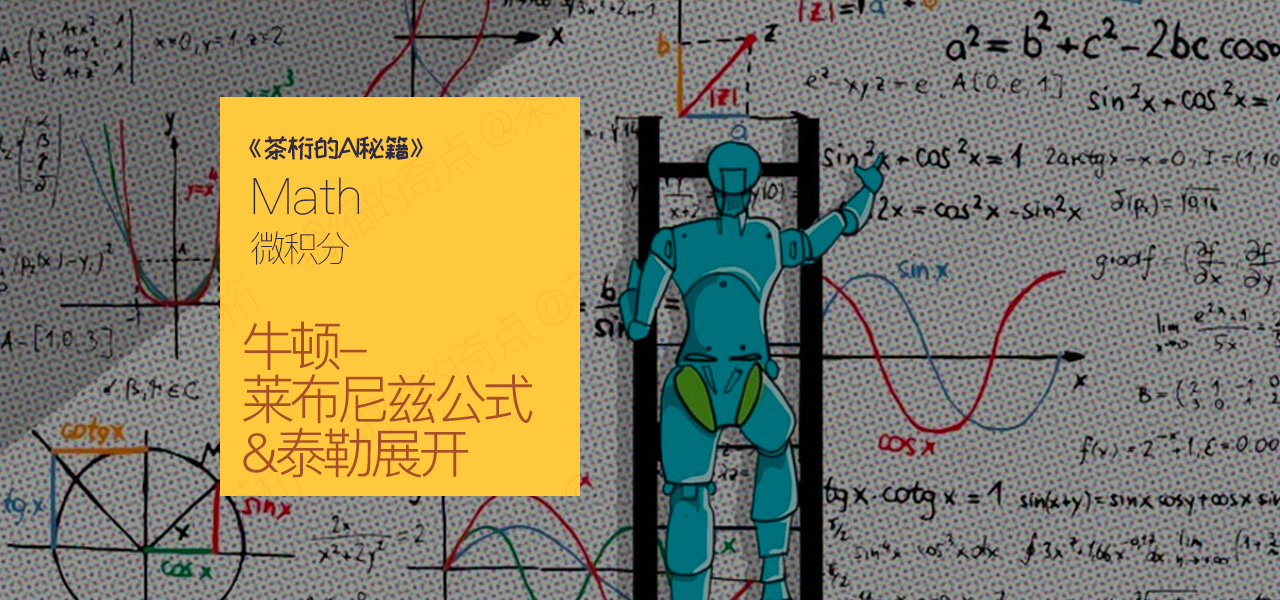
\includegraphics[width=1\linewidth]{asset/茶桁的AI秘籍_Math_13.png}
\end{figure}
\newpage

上一节课中, 我们留了一个小尾巴, 就是我让大家注意了一下这个式子: 
\begin{align*}
  x^2\vert _{x=6}-x^2 \vert _{x=1}=6^2 - 1^2 = 35
\end{align*}
这段含义就是$x^2$(在$x$等于6的时候)减去$x^2$(当$x$等于1的时候). 它的结果就是6的平方减1的平方, 它也等于35, 好神奇. 那难道说这$x^2$和$2x$之间有什么关联吗? 或者说我们把$\int_a^b2xdx$的积分写成$x^2\vert_{x=b}-x^2 \vert_{x=a}$?, 难道这两者是相等的吗?

在这里引出了微积分里面的非常重要的一个定理了: \textbf{牛顿-莱布尼兹公式}. 

\section{牛顿-莱布尼兹公式}

\textit{牛顿-莱布尼兹公式}, 我们通过一个运动学的问题去说, 它表述了怎么样的一个场景呢?

首先, 物体的初速度大小是0, 它做一个匀加速直线运动, 其加速度是$2m/sec^2$, 那么它的位移时间方程$s$就应该是$s=\frac{1}{2}at^2 = t^2$. 物理课上学过的, 有不清楚的同学可以自己搜索一下, 很好理解. 把$a$的数值带入之后, 它就等于$t^2$. 

然后我们还可以考虑, 不是做匀加速吗, 那速度和时间的方程它应该就是$ v = (s)' = 2t$. 打个比方, 比如说初速都是0, 一直做匀加速, 每过一秒速度就增加2. 所以它的函数方程就应该是$2t$. 其实也就相当于对位移求导. 就可以得到速度方程, 是物理学上面的一个常识. 

先看一下两个图像, 图\ref{fig:img14_1}是位移时间方程的图像, 图\ref{fig:img14_2}是速度时间的函数图像. 分别是$s=t^2$以及$v=2t$. 

\begin{figure}[ht]
  \begin{minipage}[t]{0.48\textwidth}
    \centering
    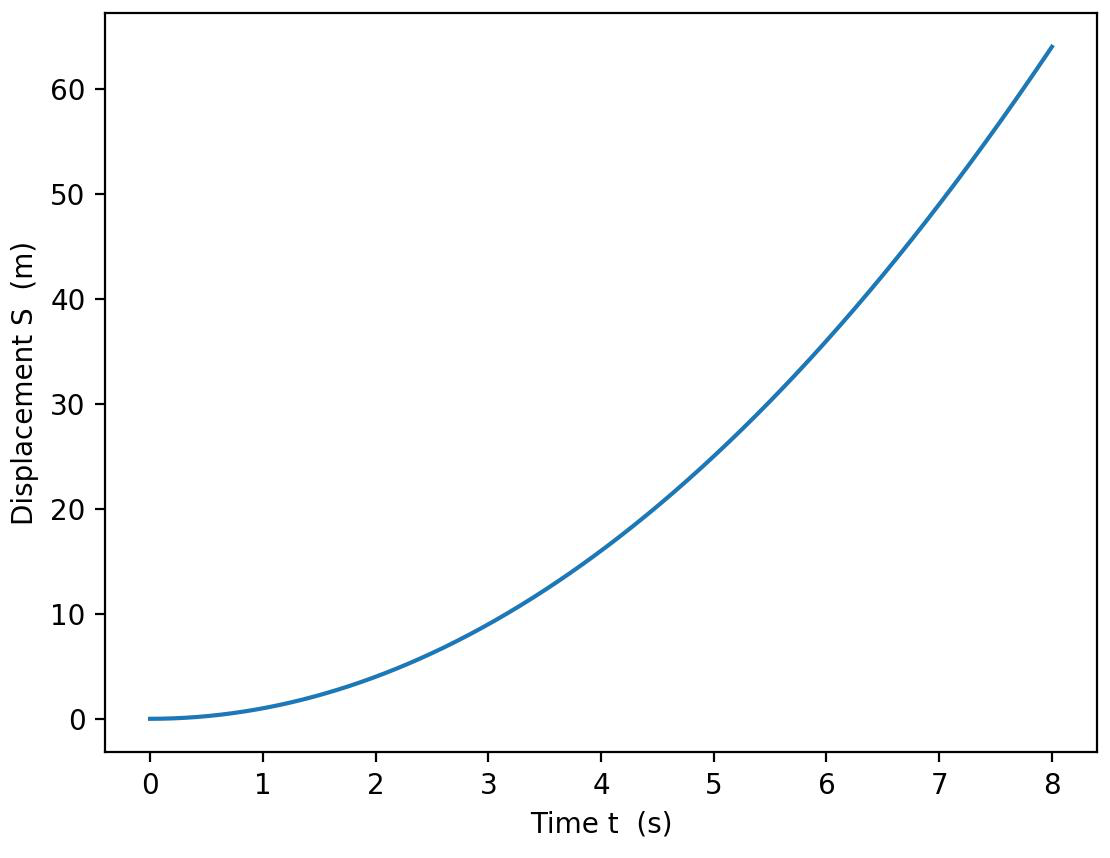
\includegraphics[width=\textwidth]{asset/20230904115319.png}
    \caption{$s=t^2$}
    \label{fig:img14_1}
  \end{minipage} %
  \hspace{1em}
  \begin{minipage}[t]{0.48\textwidth}
    \centering
    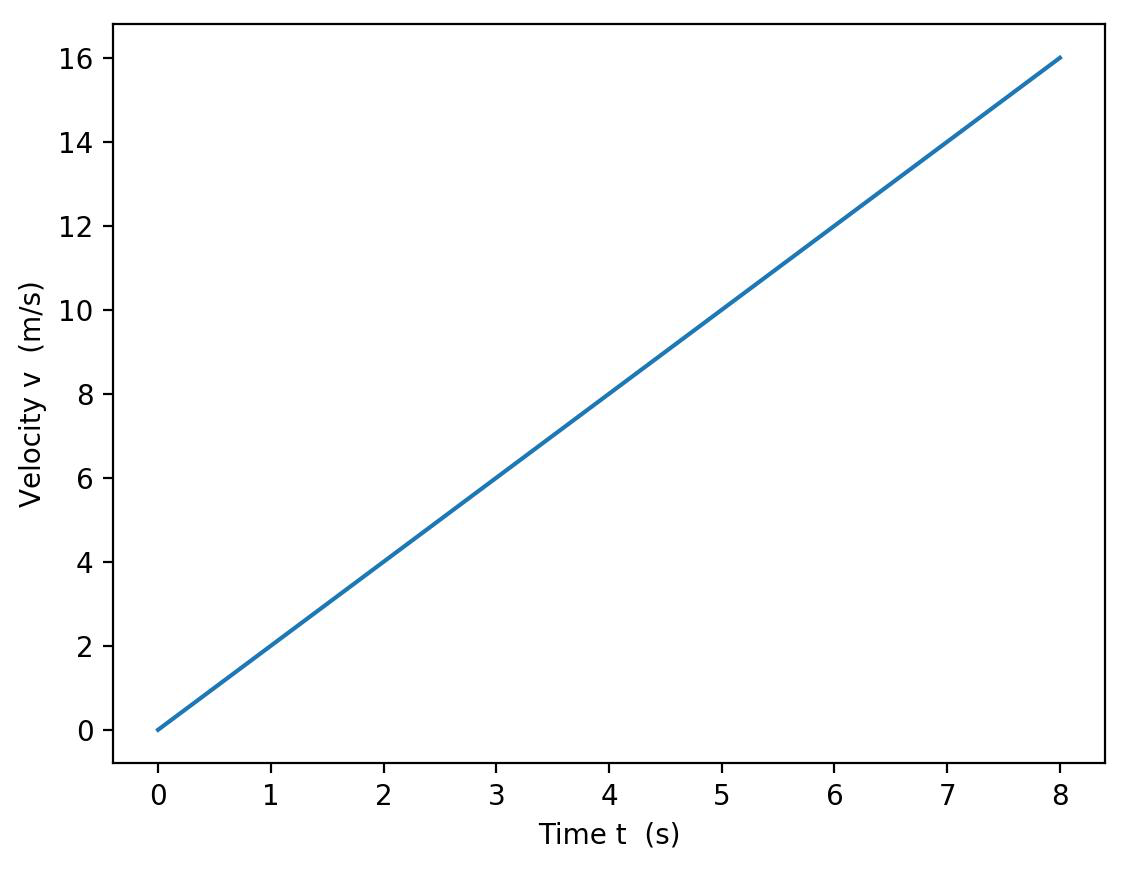
\includegraphics[width=\textwidth]{asset/20230904115338.png}
    \caption{$v=2t$}
    \label{fig:img14_2}
  \end{minipage}
\end{figure}

再来看一下这两个图所对应的几何意义. 比如说我从0秒一直到5秒, 上面位移时间图像里面它代表什么意义呢?0秒的时候在原点, 距原点的距离为0, 在5秒的时候就应该在如图的位置, $5^2$, 应该是25米, 如图\ref{fig:img14_3}: 

\begin{figure}[ht]
  \centering
  \caption{}
  \label{fig:img14_3}
  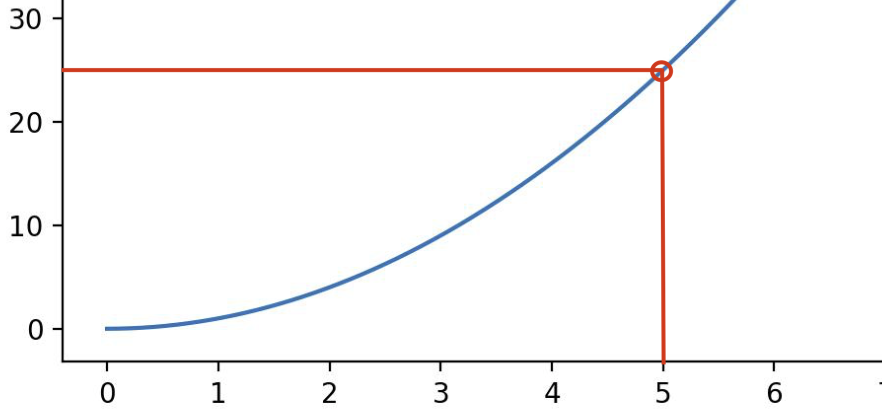
\includegraphics[width=0.5\linewidth]{asset/20230904131050.png}
\end{figure}

从0秒到5秒总共走了多远是不是就是直接拿纵坐标直接减就行了?$25-0$, 那不就是25嘛. 

同样的问题再放在速度时间方程上面来看. 横坐标是时间t, 纵坐标是速度v, 我们知道速度乘以时间就是等于路程, 或者说等于位移. 函数曲线和$x$轴围成的面积几何意义就是位移. 如果我们想通过速度时间图像去求解从0秒到5秒总共走了多远的话, 求0秒到5秒形成的三角形的面积就行. 

我们已经知道面积代表着 $v\cdot t$, 不管是矩形还是三角形, 两个数值乘在一起代表的物理含义就是位移. 所以对于速度图像而言, 我们求它从0秒到5秒走过的路程就是把从原点出发,一直到5秒, 围成的这么一个三角形的面积求出来. 如图\ref{fig:img14_4}: 

\begin{figure}[ht]
  \centering
  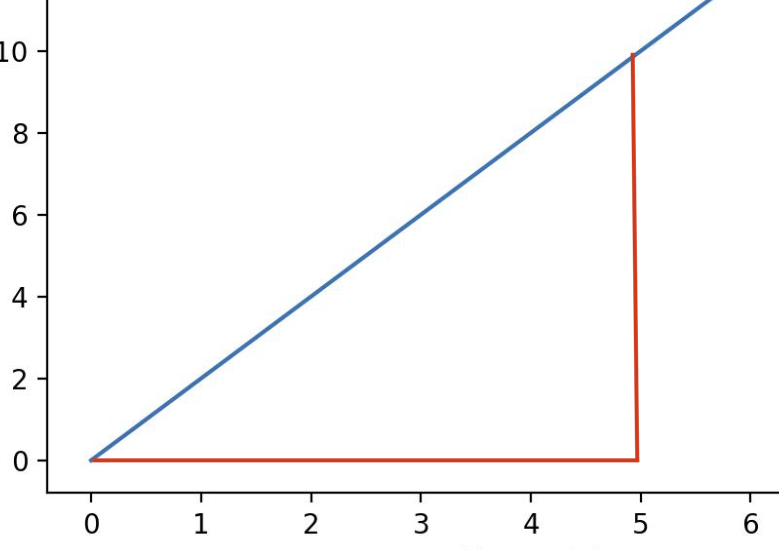
\includegraphics[width=0.5\linewidth]{asset/20230904131921.png}
  \caption{}
  \label{fig:img14_4}
\end{figure}

三角形对应的面积就是我们在这5秒内走过的位移. 

那按照几何意义来说的话, 面积怎么求呢?边长分别是5和10, 所以面积等于$\frac{1}{2} \times 5 \times 10$, 等于25. 和我们用位移时间函数所求到的结果是一模一样的, 唯一的区别就是在位移图像里面它是直接纵坐标结束值和初始值相减, 在速度图像里面是求面积. 

那我们就发现了一个非常神奇的事实: 当我们对速度函数求积分的时候, 其实就是求被积函的原函数. 

其实就是对速度函数做了一个反向求导, 从位移到速度它是一个求导过程. 从速度到位移我们暂且把它叫做反向求导, 就是回到里面逆向求导一下, 得到函数之后再减去相应的纵坐标值就可以了. 

牛顿-莱布尼兹公式非常非常的重要. 因为它告诉了我们对于积分的形式我们应该怎么样去求解, 我们来看一下定积分公式: 

\begin{align*}
  \int_a^b f(x)dx = F(x) \vert_a^b = F(b) - F(a)
\end{align*}

如果我们要求积分的话, 只需要找出$f(x)$对应的原函数, 然后把它在a点和b点的值求出来相减, 就可以得到$f(x)$从a到b之间积分的值. 

这是非常重要的一个事情, 因为它被发现之前呢其实人类是不知道怎么样处理. 虽然我知道$\int_a^b$的意义, 知道怎么求导, 但是关键我不知道怎么积. 正是因为公式的发明, 我们才知道, 原来求它原函数就行了. 

原函数的意思就是说, 比如这里$f(x)$是$2x$的话, 那它的原函数是什么样的函数求导得到了$2x$呢?就是$x^2$. 

所以我们可以看到积分其实是分成两种, 一种称为「定积分」一种称为「不定积分」. 定积分有具体的积分上下界以及具体的函数值相减, 对应的这么一个结果. 而不定积分只需要求出一个原函数就可以了. 不定积分公式如下: 

\begin{align*}
  \int f(x)dx = F(x) + C
\end{align*}

不管是定积分还是不定积分, 核心都是逆向求导, 找出原函数. 

细心的小伙伴会注意到, 在不定积分这里求出来原函数还加了一个常数$C$. 为什么要加$C$呢?难道说$f(x) = 2x$, $F(x)$是$x^2$, 又或者是$x^2 + 1$都行吗?我们可以尝试求导试一下, 确实是这样没错. 这其实是一个之前课程中教过的问题, 就是常数求导等于多少?等于0对吗?这项没有了不会体现在这里. 

所以我们反向求导的时候会给它加上一个常数$C$, 表示它的原函数不是只有一个, 是有无穷多个, 根据$C$来做区别, 但是核心的$F(x)$这一部分是一样的.

很多小伙伴求不定积分, 反向求导的时候把$F(x)$求出来就万事大吉了, 忘了加一个常数$C$. 也有的不太会加, 其实就直接写上$+C$就行. 因为你也并不知道常数是什么, $C$可以代表任何常数. 不能就光写一个$F(x)$. 

在我们定积分和不定积分的两个公式中,  $F(x)$是$f(x)$的原函数,  $C$为常数,  $a, b$是积分区间. 

来看一个例子: 求积分$\int_1^6(x^3 + 3x^2+cos x)dx$的值. 

我们从1到6积的积分, 这被积函数看着似乎很复杂的样子, 如果我们不知道牛顿-莱布尼兹公式的话就束手无策, 但是因为这两位大神特别给力, 所以现在我们只需要找出这个被积函数的原函数是什么: 

\begin{align*}
  F(x) = \frac{1}{4}x^4 + x^3 + sinx
\end{align*}

大家可能一开始会比较习惯了求导, 但是反向求导或者说求原函数的过程可能还得有一个适应的过程, 多练几遍其实就熟悉了. 

打比方说,  $x^3$, 我们想一下,三次方之前肯定是四次方, 四次方要求导拿下来肯定会有一个数字4, 那在被积函数里数字4没有了, 所以原函数肯定是有一个常数1/4, 当求导的时候, 拿下来的4和1/4抵消了, 所以在被积函数里系数才是1, 求出来导数是$x^3$. 

当前我们举的这个例子还是比较去好判断它的原函数, 有一些函数的原函数比较难去判断, 会比较复杂. 还有一点, 就是我们要知道, 这是被积函数的\textbf{一个原函数}是这样子, 因为被积函数原函数有无穷多个, 只要加上一个常数$C$, 就无穷多个. 我在这里我只是写出这么一个, 就是常数为0的情况. 

\begin{align*}
  & \int_1^6(x^3 + 3x^2+cosx)dx = F(x)\vert_1^6 \\
  & = (\frac{1}{4}\times 6^4 + 6^3 +sin6) - (\frac{1}{4} \times 1^4 + 1^3 + sin1) \\
  & \cong 1510.84
\end{align*}

所以呢积分值就对应着原函数在1和6处, 这两个点的取值的一个差. 算了一下, 近似值呢是$1510.84$, 是一个无限小数. 

这里还有一个地方要给大家说明一下, 大家看到$sin6$, 还有后面的$sin1$, 并不是代表着6度, 它并不是代表着我们平时理解的角度. 我们可以注意到无论是6还是1, 右上角都没有代表\textbf{度}的小圆圈\textbf{$^\circ$}, 因为它本身就不是角度, 代表的是弧度. 

弧度和角度怎么样去换算呢?就是$2\pi$, $2\pi$等于$360^\circ$, $\pi$ 就等于$180^\circ$, 换算的话, 1弧度 = $(180 / \pi)^\circ$,  $1^\circ$=$\pi / 180\mbox{弧度}$ . 大家这里可以了解一下. 

\section{牛顿-莱布尼兹公式的意义}

那牛顿-莱布尼兹公式对于我们有什么样的意义呢?

首先, 他提供了求积分问题的一个非常有效的办法, 我们可以通过方向求导得出被积函数的原函数;并且将复杂的积分运算转化为简单的加减运算. 

为什么说积分运算是一个非常复杂的运算, 就是因为如果我们没有牛顿-莱布尼兹公式的话, 如果要去计算积分唯一的办法只有一开始说的, 通过画无限多个矩形去逼近它, 积分这一种方式去做. 而划分的过程就太复杂, 这跟你划分的多精细还有关. 而且关键最后得到结果还不是一个很准确的值, 只是一个近似值, 永远只是一个近似值, 你永远达不到它积分的值. 而公式将复杂的积分运算化解成了简单的这种加减运算. 

第二个, 它架起了微分学和积分学之间的一个桥梁. 历史上其实微分学和积分学一开始是独立发展的. 那个时候科学家是不知道这两个东西是有联系的, 并没有意识到一个正向一个反向过来. 自从牛顿-莱布尼兹公式提出之后, 微分学和积分学才被称为了微积分. 

正因为上面的这些重要性, 牛顿-莱布尼兹公式也被称为了微积分基本定理. 这是一个很高的荣誉, 整个微积分的基本定理. 

接下来, 再给大家一个小知识点: 

我们考虑, 一个直恒为正的函数, 也就是不存在图像在$x$轴下方出现负面积的情况. 

比图\ref{fig:img14_5}这样, 函数值恒为正. 如果是函数的话, 考虑它的几何意义是什么. 就是函数图像以及$x$轴所围成的面积, 通过积分求出来的就是面积. 

\begin{figure}[ht]
  \centering
  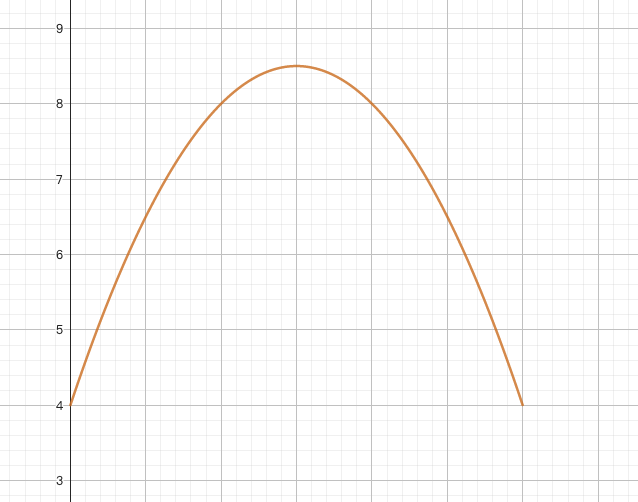
\includegraphics[width=0.5\linewidth]{asset/20230904153345.png}
  \caption{}
  \label{fig:img14_5}
\end{figure}

那问题来了, 我们通过积分运算求出来的值是它和$x$轴围成的面积的准确值, 还是说它是一个极度逼近的一个近似值?准确值什么意思, 就是面积被求出来了, 一点点都不差, 正好是这么多. 而极度逼近的近似值就是可以无限的逼近, 误差非常非常小, 但是还是不相等, 还是有一点点误差. 

其实答案是准确值. 

为什么我在这里提出这么一个问题?因为我还记得上高中的时候, 发现我周围的同学很多人以为是一个极度逼近的近似值, 而不是一个准确值. 就跟那个极限的概念一样, 很多人觉得它是一个无限逼近但永远达不到的这么一个过程. 

\textbf{积分求出来的, 就是一个准确值. 它面积是多少, 通过积分求出来就是多少}, 大家这点要记住. 

\section{泰勒展开}

接着, 是我们微积分里最后一部分: 泰勒展开. 是不是看到这里大家都舒一口气?万里长征终于来到最后一站了, 当然还是会有些公式. 

首先, 我们通过微积分基本定理可知下面的式子: 

\begin{align*}
  f(x) - f(a)  = \int_a^xf'(t_1)dt_1 \implies f(x) = f(a) + \int_a^xf'(t_1)dt_1
\end{align*}

这里被积函数用$f'(x)$表示了, 原函数用$f(x)$表示. 然后我们稍微做一下变形, 就能得到$f(x) = f(a) + \int_a^xf'(t_1)dt_1$. 

然后再对$f'(t_1)$做同样的处理, 就是$f'(t_1)$是关于$t_1$的一个函数, 导函数它也是一个函数, 就像我们之前说过的, 导数可以求很多阶, 只要你n阶可导的话, 你一直可以求到n阶导数. 所以求了一次导之后, 它仍然可能是一个量的函数. 

我们再做同样的处理: 

\begin{align*}
  f(x) = f(a) + \int_a^xf'(a)dt_1 + \int_a^x \int_a^{t_1} f''(t_2)dt_2dt_1
\end{align*}

就是把上一个式子中结果里的$f'(t_1)$看作成它所在式子中最前方的$f(x)$, 其实做的就是这么一个事情. 如果大家式子觉得看着脑壳疼可以不用去看. 我就告诉你, 就是把$f'(t_1)$看作了$f(x)$一样, 然后套用一下$f(x) - f(a)  = \int_a^xf'(t_1)dt_1 $这个式子去做. 

头晕了吗?别急, 往下看, 往下看你就会更晕了, 接着, 我们在对上面得到的式子中的$f''(t_2)$继续做同样的处理: 

\begin{align*}
  & f(x) \\ & = f(a)+\int_a^xf'(a)dt_1 + \int_a^x \int_a^{t_1} f''(a)dt_2dt_1+\int_a^x\int_a^{t_1}\int_a^{t_2}f'''(t_3)dt_1dt_2dt_3
\end{align*}

这里呢, 其实就是把$f''(t_2)$同样看作$f(x)$, 然后得到结果, 就是这么一大长串. 双重积分、三重积分;你想要几重都可以, 看你自己乐意. 

那我们做这些有啥意义呢?别急, 接着往下看. 

首先, 我们先来看一下形式, 先别管这后面这一项, 后面一项它是跟$t_3$有关的,$t_3$是一个自变量, 不是一个常数. 

我们来看一下前面, $f(a)$是一个常数了, $f'(a)$是一个常数了,$f''(a)$是一个常数了. 那不就是$f(x) = a$处函数值、一阶导数、二阶导数, 不都是常数吗?所以$f(a), f'(a), f''(a)$这三个均为常数, 我们可以得到什么?直接对它做积分: 

\begin{align*}
\int_a^xf'(a)dt_1 = \frac{f'(a)}{1}(x-a)
\end{align*}

这里, 可以把$f'(a)$用$C$来代替, 但我们还是先给它保留一下:$\frac{f'(a)}{1}$. 

我们可以这么看, 先别管$f'(a)$, 把这项给拿掉, 就看做它系数是1, 就是积分a到$x$, 乘上1,  然后乘上$dt_1$. 

什么东西求出来它的导数是1呢?不就是$f(x) = x$, $t_1 = x$的时候、$t_1 = a$的时候, 它两相减乘出来的结果, 再乘上常数$f'(a)$, 在这里它除以1是我人为加的. 如果计算的话, 不会有除以1这一步, 那我为什么要人为加这么一个呢?我们接着往下看:

\begin{align*}
  \int_a^x\int_a^{t_1}f''(a)dt_2dt_1 & = \int_a^x \frac{f''(a)}{1}(t_1 - a)dt_1 \\
  & = \frac{f''(a)}{1 \times 2}(x-a)^2
\end{align*}

求二重积分怎么求?我们从里到外一步一步的求, 我们先看这部分: 

\[\int_a^{t_1}f''(a)dt_2\]

不然两个一块看你绝对脑壳疼, 而且也反应不过来. 

这一部分求积分不就和上方的式子类似吗, 求出来结果就是$\frac{f''(a)}{1}(t_1 - a)$, 和上面类似, 只不过就是表现形式上面, 符号上面有一些差别. 

当我们做完了这些之后, 我们再来求这部分: $\int_a^x \frac{f''(a)}{1}(t_1 - a)dt_1$, 双重积分我们就一层一层来,别想一口吃个胖子, 想一下子就把两层积分全给做了. 那这个时候, $\frac{f''(a)}{1}$是一个常数, 然后$t_1$是自变量的一次, $a$是一个常数. 所以我们求出来最终结果. $t_1-a$这部分的原函数, 写成$\frac{1}{2}t_1^2 - at_1$. 再往里面带, 当它等于a的时候什么值, 当$t_1$等于$x$的时候什么值. 

注意, 这里的$x$ 它就不再是我们惯常表示的那个自变量了, 这里$x$我们可以把它当成一个常数. 

通过我们牛顿-莱布尼兹公式可以算出来双重积分求出来结果:$\frac{f''(a)}{1 \times 2}(x-a)^2$. 

然后我们接下来再来看一下, 我们一直这样做下去会怎样. 一直做下去, 那他四重积分又出来了, 之后是五重、六重, 一直到n重都能出来. 在n重之前的这些积分, 不管多少重, 它这里面都是一个常数. 所以我们在这里就可以得到: 

\begin{align*}
  & f(x) \\
  & = f(a) + \frac{f'(a)}{1!}(x-a) + \frac{f''(a)}{2!}(x-a)^2+...+\frac{f^{(n)}(a)}{n!}(x-a)^n+R_n(x)
\end{align*}

只要我们一直做下去,就会发现$f(x)$可以表示成这种形式. 它在某一点的函数值, 这一点的一阶导、二阶导、三阶导, 都乘上一个多项式, 一直到$n$次的多项式, 然后再除以n的阶乘. 

阶乘是什么意思大家都应该知道吧?我们拿5举例,  5的阶乘就是$1\times 2 \times 3 \times 4 \times 5$, 多少的阶乘就是从1一直乘到多少个数. 阶层的增长率其实是超过指数函数的, 它的增长速度是远超过指数函数的, 阶乘是一个很可怕的数. 

当然, 在数学上面如果你要表示非常大的数, 可以用高德纳数来表示, 这里就不展开说了. 

最后, 我们还拖了一个小尾巴, $R_n(x)$为什么没有写了,如果它写的话它是套了n重积分的一个形式. 

这里我们就把函数用这种形式来表示, 那形式有什么意义?其意义非常大, 我们一个一个来看: 

\textbf{不管是什么样形式的函数, 都可以通过多项式函数来拟合}. 多项式函数: 易于计算, 可以快速获得结果. 

比如$cosx$,  当$x$为30度, 45度, 90度的时候, 我们都可以进行计算. 但是当x为$37^\circ$, $38.89^\circ$, $\pi/2$, 你还能算出来吗?人和机器都不行. 算这些函数都是通过「泰勒展开」来计算的. 把他们化成这种形式: 就是我们上面最终的$f(x)$得到的形式去计算的, 通过计算多项式函数来做. 

所以大家不要以为计算机啊很牛逼, 其实它在智能程度远逊于人类, 它只能做一些非常简单的二进式的加减法, 什么$0+1, \quad 1+0, \quad 1\times 1$这种东西. 但是它可以通过把复杂函数转换成多项式, 通过强大的算力快速的告诉我们结果, 计算机就是这样去计算. 

包括大家在中学的时候应该用过一个中学数学用表, 在上面会看到不同的函数, 在$x$等于几的时候都会有一个近似值. 那时候是不是很好奇值咋算的, 我那时候就好奇过. 那时候我反正是想不明白这东西怎么算. 后来查资料就发现是通过泰勒展开算出来的, 就是通过这种方式. 

\textcolor{red}{所有的复杂函数都是用泰勒展开转换成多项式函数计算的.}

\textbf{泰勒展开也是有一个适用范围的}. 举一个例子: $\frac{1}{1-x} = 1+x+x^2+x^3+o(x^3)$

这个函数, 不是对任意的$x$都成立, 比如如果我$x$等于10的话, 左边是一个负数了,但是你看右边是一个非常大的一个正数, 这根本是不可能的. 这还引发过数学史上非常有名的一个悖论. 所以泰勒展开它是有一个适用范围的. 对于上面这个例子而言, 它的适用范围就是1, 它的收敛半径就是1. 

有一种泰勒展开比较特殊, 就是\textbf{令多重积分里这些a等于0的时候, 这种泰勒展开被称为麦克劳林展开}. 

我们来看一个例子, 来看一下它到底是否像说的那么厉害. 

\textit{例: 求函数$f(x) = e^x$在$x=1$时的值}

当我们拿到这个函数的时候, 感觉都没办法去做, e的值都不知道. 其实就是让我们求e的值. 

由函数的麦克劳林展开式, 我们可以得到:

\[
  f(x) = e^x \cong 1 + \frac{1}{1!}x^1 + \frac{1}{2!}x^2 + \frac{1}{3!}x^3 +\frac{1}{4!}x^4 + \frac{1}{5!}x^5
\]

我们这里就先精确到$x$的5次方. 

我们最终得到结果: 

\begin{align*}
  f(1) = e^x & \cong 1 + \frac{1}{1!}x^1 + \frac{1}{2!}x^2 + \frac{1}{3!}x^3 +\frac{1}{4!}x^4 + \frac{1}{5!}x^5 \\
  & = 2.7167
\end{align*}

通过查表, e的值是多少? 是$e^1 = e = 2.71828...$, 一直循环下去. 我们会发现仅仅是通过简单的四则运算, 再加上简单的乘方运算, 乘方当然也可以转化为乘法运算. 就计算出了一个非常复杂函数的值, 泰勒展开的威力可见一般. 

在计算机去处理的时候, 其实它没有我们聪明, 人做不到事情它也做不到, 只能转换成这些多项式然后去计算. 靠的是它强大的算力, 可能把小数点的位数给精确到多少位多少位, 再交给我们去查, 仅此而已. 

那我们如何理解泰勒展开?其实泰勒展开是可以用一系列的多项式函数来拟合任意一个函数, 它拟合的道理是什么?我们看图\ref{fig:img14_6}, 红色的线代表了我们要拟合的函数, 锯齿状的绿色曲线代表了我们拟合的效果. 泰勒展开就是想用一个函数模拟另外一个. 模拟不仅仅代表着在某些点的坐标, 或者说函数值相同;更代表了在这些点的一阶变化率相同, 二阶变化率一直到n阶变化率都相同. 

\begin{figure}[ht]
  \centering
  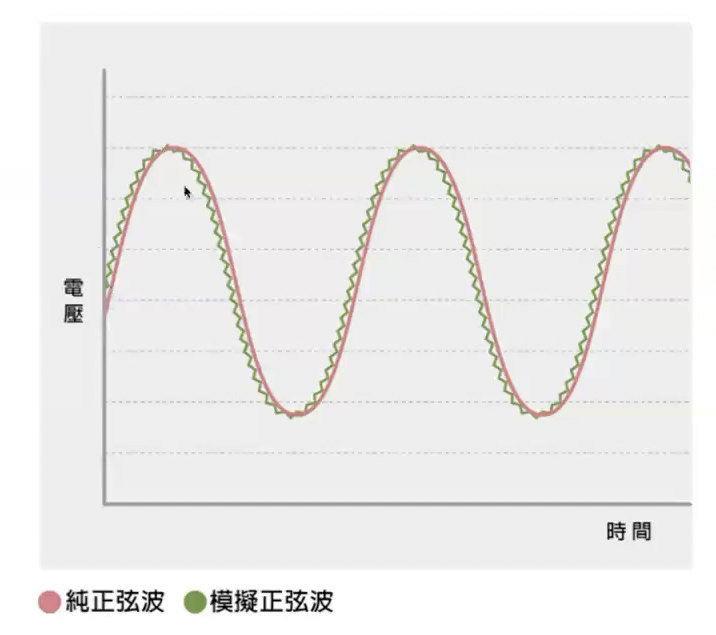
\includegraphics[width=0.8\linewidth]{asset/20230904180649.png}
  \caption{}
  \label{fig:img14_6}
\end{figure}

也就是两个函数如果非常接近了, 非常趋于相同了. 那应该说不光在某些点函数值相同, 在这些点的各阶的变化率对应的情况也相同. 

就像两个赛车在比赛一样, 不是哪些位置他们俩的速度相同, 还得比他们在哪些位置的加速度是否也相同, 这样他们运动曲线才是一样的. 也就是说, 如果两个函数$f(x)$和$g(x)$相同, 那么: 

\begin{align*}
  & f(x) = g(x) \\
  & f'(x) = g'(x) \\
  & f''(x) = g''(x) \\
  & ... \\
  & f^{(n)}(x) = g^{(n)}(x) \\
  & \mbox{各阶的变化情况相同}
\end{align*}

\section{结束语}

以泰勒展开为结束点, 今天的课程到这里也就结束了. 微积分相关的内容到这里就全部讲完了, 当然所讲的这些内容, 在熟悉之后应付人工智能是能应付了, 但是远远不是微积分的所有内容, 并且讲的也并不细致. 所以不要将我所讲的这些内容当作正规的数学教材. 如果是为了去理解和学习数学, 那么就当作我给你开了一个窗, 入门的话, 还需要正规的数学教材去系统的好好学一下. 

对于只是希望进入人工智能大门的小伙伴, 要记得我一开始所说的, 微积分这部分内容体系虽然很庞大, 但是最核心的还是\textbf{导数}和\textbf{链式法则}. 当然在神经网络里面导数大多数情况是\textbf{以偏导数的形式存在}. 我们用\textbf{梯度下降算法}去优化神经网络. 